Policy-based design \cite{Alexandrescu:2001:MCD} assemble a 
class (called \emph{host}) with complex behavior out of many 
little behaviors (called \emph{policies}). Each policy establishes
an interface pertaining to a specific behavior.
Based on this design, we implement a subdivision solution as 
a \emph{refinement function} parameterized with the 
\emph{stencils}. The host, i.e.\ the refinement function,
conducts the \tr\ and maintains the stencils. The policy,
i.e.\ the stencil, attends the \gm . By mixing and matching
the host and policy, a combinatory library of the subdivisions
can be constructed. 

In the following paragraph, we implement the Catmull-Clark 
subdivision and Doo-Sabin subdivision based on the 
policy-based design. For the sake of simplicity, all 
namespaces, template declarations
and typedefs have be excluded. The sample codes are only
given for illustration purposes.

A Catmull-Clark subdivision function is structured 
as a \emph{primal quadralization function} parameterized 
with the \emph{Catmull-Clark stencil rules}.
\begin{lstlisting}
void CatmullClark_subdivision(Polyhedron& p) {
  quadralize_polyhedron<CatmullClark_rule<Polyhedron>>(p);
}

class CatmullClark_rule {
public:
  void facet_rule(Facet_handle facet, Point& pt);
  void edge_rule(Halfedge_handle edge, Point& pt);
  void vertex_rule(Vertex_handle vertex, Point& pt);
};
\end{lstlisting}
The \lstinline!quadralize_polyhedron<>()! is the host function
refining the input mesh
and the \lstinline!CatmullClark_rule!
is the policy class applying the Catmull-Clark stencils. 
The refinement host calls the policy
functions while maintaining the correspondence of stencils, 
i.e.\ the submesh centered as the given facet, edge, or
vertex handle, and the smoothing point.
Different refinement scheme may require a 
different set of stencils. A PQQ scheme needs
facet-, edge- and vertex-stencils whereas a DQQ scheme 
only need the corner-stencils (Figure \ref{fig:RefMap}).

\noindent\textbf{Geometry Policies}.
Inside a policy, applying stencil is simplified as 
the mesh traversal of only a 1-ring neighborhood. 
Following example shows the policy of facet-stencil 
in the Catmull-Clark subdivision.
\begin{lstlisting}
void facet_rule(Facet_handle facet, Point& pt) {
  Halfedge_around_facet_circulator hcir = facet->facet_begin();
  Vector vec = hcir->vertex()->point() - CGAL::ORIGIN;
  ++hcir;
  do {
    vec = vec + hcir->vertex()->point();
  } while (++hcir != facet->facet_begin());
  pt = CGAL::ORIGIN + vec/circulator_size(hcir);
}
\end{lstlisting}
The \lstinline!Facet_handle facet! points to the 
center facet of the stencil and the \lstinline!Point& pt! 
specifies the smoothing vertex. For this specific stencil, 
we compute the centroid with a loop based on a circulator 
over the halfedges surrounding a facet. The CGAL kernel 
geometry, i.e. Points and Vectors computation, is used. 
Though for a specialized kernel, special computation may be 
applied in user-defined policies.
 
\noindent\textbf{The refinement host: Euler operations}.
Implementing a topology refinement is a rather complex job. One
approach is to encode the refinement into \emph{a sequence of Euler
operations}. For Catmull-Clark subdivision, the refinement is encoded
as edge-vertex insertions, edge insertion between two neighboring
edge-vertices, facet-vertex insertion on the inserted edge, and then
edge insertions between the facet-vertex and the edge-vertices. 
The Euler sequence is demonstrated in Figure \ref{fig:CCRefinement}. 
Note that the vertex and edge insertions can be easily 
implemented based on the Euler operations supported by \cgalpoly.
\begin{figure}
  \centering
  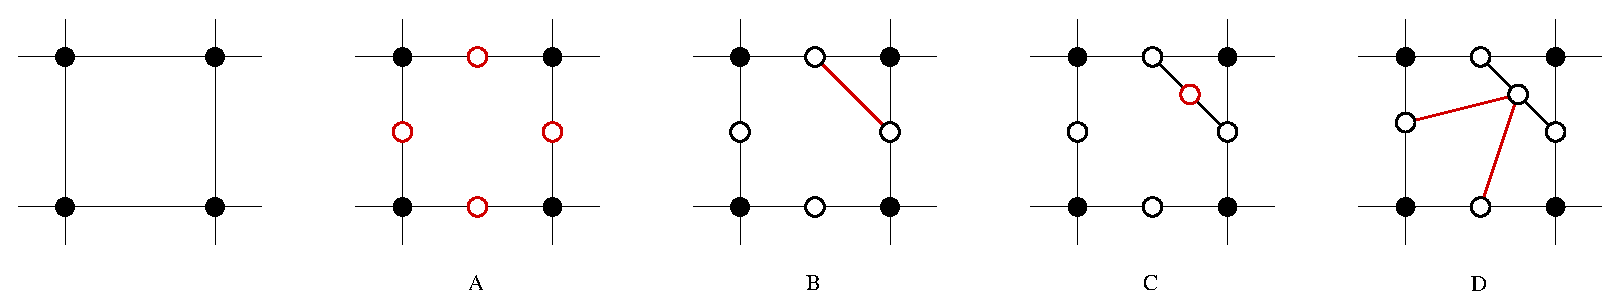
\epsfig{file=figs/CCRefinement.eps, width=7cm}
  \caption{A PQQ refinement of a facet is encoded into a sequence of
  vertex insertions and edge insertions. Red indicates the inserted
  vertices and edges in each step.}
  \label{fig:CCRefinement}
\end{figure}

The stencil correspondence of the refinement is assured
by matching the \emph{traversal sequences} of the mesh. 
The refinement host has a two pass, hence two traversal, 
algorithm. The first pass generates the points by 
calling the policies. The second pass
refines the mesh with a sequence of the Euler operations.
The points generated in the first pass are stored in a
point buffer in the order of the stencil 
traversal. The sequence of the vertex insertions 
is maintained to match the the stencil traversal, i.e.\ 
the storage order of the point buffer. It assures 
the stencil correspondence of the refinement.

\noindent\textbf{The refinement host: modifier callback mechanism}.
Most primal refinement schemes can be translated into a sequence of
Euler operations. Though dual schemes, e.g.\ Doo-Sabin subdivision,
have no simple translation of Euler operations. A sequence
of Euler operations for a DQQ scheme consists of two times 
of the midedge refinement \cite{Peters:1997:SSS} and 
result an inefficient implementation. This multipass 
refinement scheme, called subdivision operator factorization, 
is proposed in \cite{Peter:2003:CPDSS}.
To support such schemes efficiently, we use the modifier 
callback mechanism of \cgalpoly\ to rebuild the mesh
connectivity. In addition to the points buffer, we
also create a facet list based on the source mesh. Note that in a DQQ
scheme, every new facet corresponds to a vertex, edge or facet. The
combination of the points buffer and facet list represents a
facet-vertex index list which indexes the vertices and enumerates each
facet as an index sequence. A modifier creating a polyhedron from a
facet-vertex index list is then a simple task.
\begin{lstlisting}
pb.begin_surface(num_point, num_facet); {
  for (int i = 0; i < num_point; ++i) 
    pb.add_vertex(Point(point_buffer[i*3+0], 
	          point_buffer[i*3+1], 
	          point_buffer[i*3+2]));	
  for (int i = 0; i < num_facet; ++i) {
    pb.begin_facet(); {
      for (int n = 0; n < facet_buffer[i][0]; ++n)
      pb.add_vertex_to_facet(facet_buffer[i][n+1]);
    }
    pb.end_facet();
  }
}
pb.end_surface();
\end{lstlisting}


\begin{figure}
  \centering
  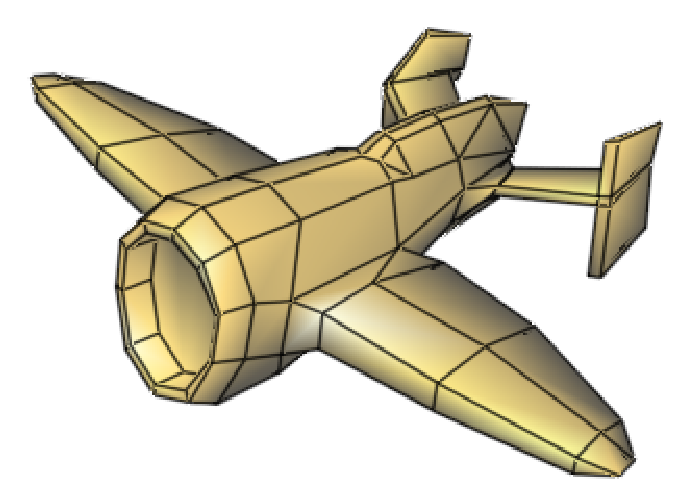
\epsfig{file=figs/plane0.eps, width=3.5cm}\\
  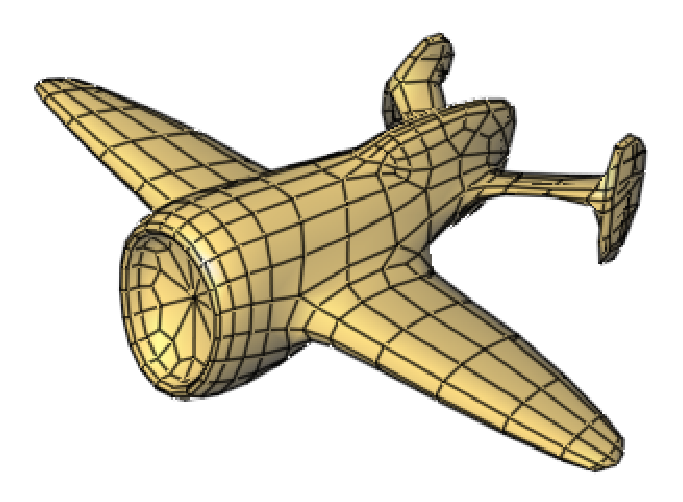
\epsfig{file=figs/planeCC1.eps, width=3.5cm}
  \vspace{0.3cm}
  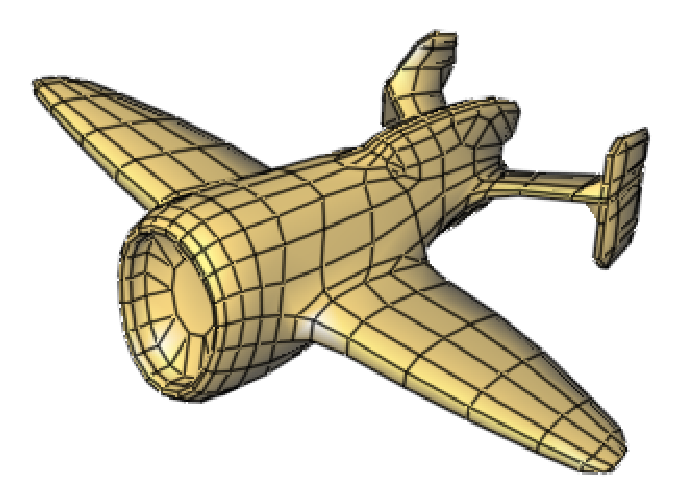
\epsfig{file=figs/planeDS1.eps, width=3.5cm}\\
  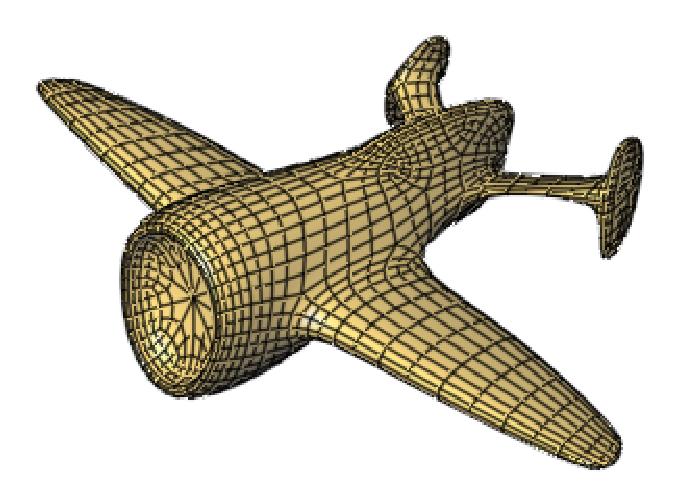
\epsfig{file=figs/planeCC2.eps, width=3.5cm}
  \vspace{0.3cm}
  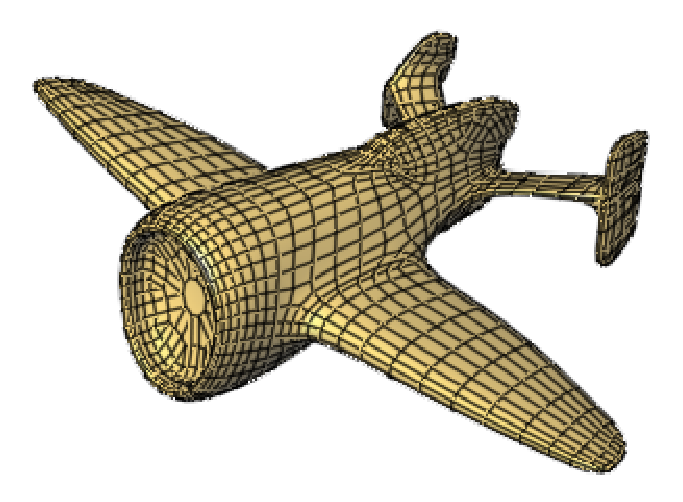
\epsfig{file=figs/planeDS2.eps, width=3.5cm}\\
  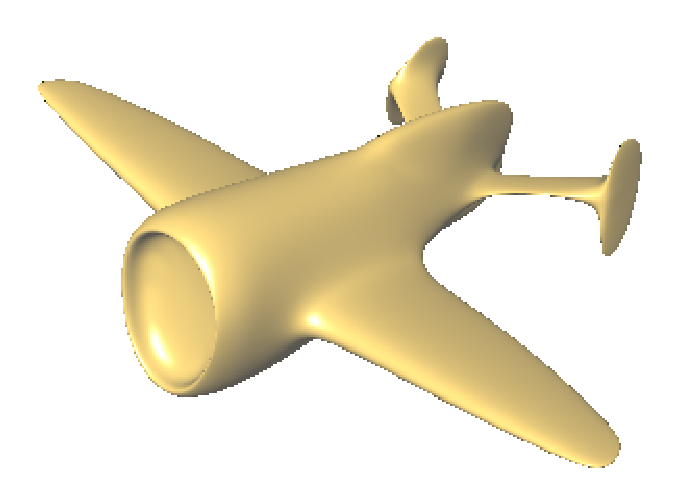
\epsfig{file=figs/planeCC.eps, width=3.5cm}
  \vspace{0.3cm}
  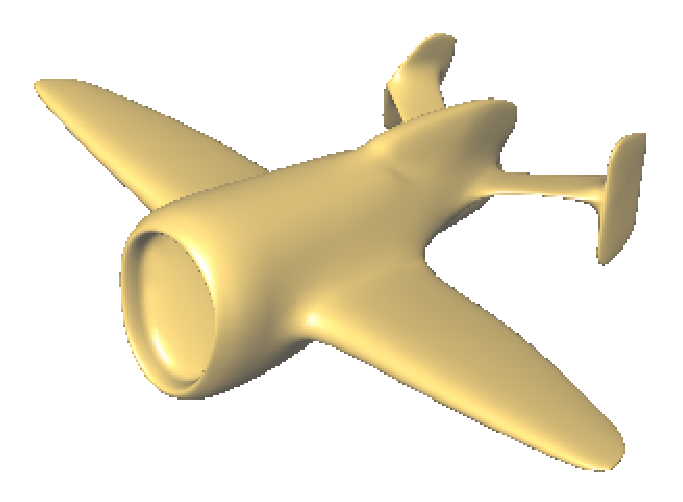
\epsfig{file=figs/planeDS.eps, width=3.5cm}
  \caption{ With the input plohedron (first raw), 
  the subdivision sequence of the 
  the Catmull-Clark subdivision (\IL) and
  the Doo-Sabin subdiviison (\IR).}
  \label{fig:SubExample}
\end{figure}

Our subdivision solution, decoupling the geometry rules from the
refinement, grants users flexible control of the stencils.
Variants of the subdivisions can be devised by simply mixing
and matching the refinement host and geometry policies. As 
our solution is not restricted by the 
mesh configurations (in contrast to the quad-tree or patch-based 
implementation), subdivision pipeline is easily supported
as a composite function like
\begin{lstlisting}
void MySubdivision(Polyhedron& p) {
  quadralize_polyhedron<Myrule_1<Polyhedron>>(p);
  dualize_polyhedron<Myrule_2<Polyhedron>>(p);
} 
\end{lstlisting}

More importantly, our solution accepts a user-specialized 
polyhedron. No special flag or attribute is required 
to assist the \tr . This generality make our solution 
naturally fit in a modeling pipeline or a multipass modeling 
environment. Though in some application, efficiency is more
important than flexibility, a tight-coupled implementation
of $\sqrt{3}$ is introduced in next section.

%TODO: since the writing memory is not overlapped, multi-threaded
%supporting is easily done.

%TODO: trade-off between generic and efficient.
 
